\documentclass[11pt]{article}
\usepackage[paperwidth=16cm,paperheight=19cm,margin=1.2cm]{geometry}
\usepackage{tikz,graphicx,booktabs,xcolor}
\definecolor{accent}{HTML}{315FD6}
\pagestyle{empty}
\setlength{\parindent}{0pt}
\begin{document}
{\LARGE\bfseries TeXAstra}\par
\smallskip
Write ideas. See them take shape.

\medskip
\textbf{Text}\par
The result is clear.
\[ E = mc^{2} \]

\textbf{TikZ}\par
\begin{center}
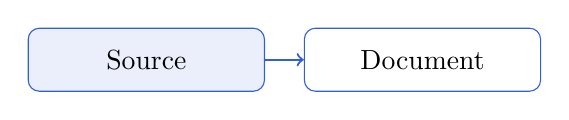
\begin{tikzpicture}
  \node[draw=accent,rounded corners,fill=accent!10,
    minimum width=3cm,minimum height=0.8cm] (a) {Source};
  \node[draw=accent,rounded corners,right=2cm,
    minimum width=3cm,minimum height=0.8cm] (b) {Document};
  \draw[->,thick,accent] (a) -- (b);
\end{tikzpicture}
\end{center}

\textbf{Figure}\par
\begin{center}
  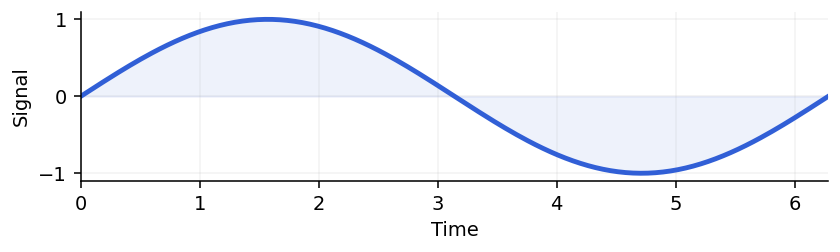
\includegraphics[width=0.70\linewidth]{signal.png}
\end{center}

\textbf{Table}\par
\begin{center}
\begin{tabular}{lr}
\toprule
Method & Score \\
\midrule
Baseline & 82 \\
TeXAstra & 95 \\
\bottomrule
\end{tabular}
\end{center}
\end{document}
